%!TEX root = thesis.tex
\chapter{Классические методы оценки стоимости Американского опциона} % (fold)
\label{cha:classic_approaches_to_option_pricing}

Cамый наивный способ оценить стоимость Американского опциона --- это промоделировать множество возможных траекторий базового актива, посчитать максимальную выплату по опциону в каждом из этих случаев (как максимум из значений $h_t(X_t)$ на промоделированной траектории $\left\{ X_t \right\}_{t \in \Tau}$) и усреднить результаты по всем промоделированным траекториям. Это классический метод Монте-Карло. Как будет видно далее (в разделе \ref{sec:results:classical_approaches}), дисперсия наивного Монте-Карло для этой задачи слишком велика.

Все рассмотренные далее способы --- это различные попытки уменьшить дисперсию наивного варианта путём увеличения числа моделируемых траекторий. 

\section{Случайные деревья} % (fold)
\label{sec:classic_approaches:tree_estimator}

Метод случайного дерева основан на моделировании цепи $X_0, X_1, \ldots X_n$ состояний актива. Зафиксируем параметр ветвления $b$. Из исходного состояния $X_0$ смоделируем $b$ независимых между собой следующих состояний $X_1^1, X_1^2, \ldots X_1^b$, все с условием $X_0$. Для каждого $X_1^i$ снова смоделируем $b$ независимых между собой последующих состояний $X_2^{i1}, \ldots X_2^{ib}$. На $m$-ом шаге будем иметь $b^m$ состояний, и это и есть источник основного недостатка этого метода --- времени работы порядка $O(b^m)$. Схема приведена на рис. \ref{fig:exponential_tree}.
\begin{figure}[b]
    \centering
    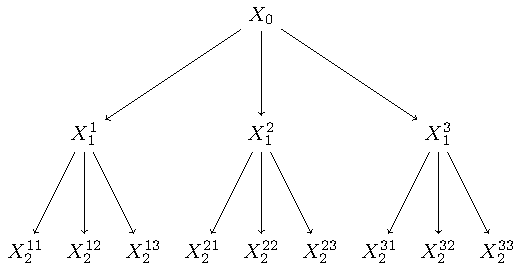
\includegraphics{exponential_tree.pdf}
    \caption{Случайное дерево для $b = 3$ и $m = 2$}
    \label{fig:exponential_tree}
\end{figure}

В \cite{Broadie1997} предложены оценки для $V_0\left(X_0\right)$ сверху ($\hat{V}_0$) и снизу ($\hat{v}_0$):
\begin{equation}\label{eq:upper}
\begin{aligned}
    \hat{V}_m^{j_1 \ldots j_m} &= h_m\left(X_m^{j_1 \ldots j_m}\right), \\
    \hat{V}_i^{j_1 \ldots j_i} &= \max \left\lbrace h_i \left( X_i^{j_1 \ldots j_i} \right), \frac{1}{b} \sum_{j = 1}^b \hat{V}_{i+1}^{j_1 \ldots j_i j}\right\rbrace,
\end{aligned}\end{equation}
\begin{equation}\label{eq:lower}
\begin{aligned}
    \hat{v}_m^{j_1 j_2 \cdots j_m} &= h\left( X_m^{j_1 j_2 \cdots j_m}\right), \\
    \hat{v}_{ik}^{j_1 j_2 \cdots j_i} &= \left\lbrace
                \begin{array}{l l}
                    h\left( X_i^{j_1 j_2 \cdots j_i}\right), & \, \text{если } \frac{1}{b-1}\sum_{j=1, j\not= k}^b \hat{v}_{i+1}^{j_1 j_2 \cdots j_i j} \leq h\left(X_i^{j_1 j_2 \cdots j_i}\right), \\
                    \hat{v}_{i+1}^{j_1 j_2 \cdots j_i k}, & \, \text{иначе}
                \end{array}\right. \\
    \hat{v}_i^{j_1 j_2 \cdots j_i} &= \frac{1}{b}\sum_{k=1}^b \hat{v}_{ik}^{j_1 j_2 \cdots j_i}.
\end{aligned}\end{equation}

В этой же работе доказаны их состоятельность, смещённость и асимптотическая несмещённость. Так, если $\exists\: p' > 1: \forall t \in \Tau \quad \E\left[ \abs{h_t(X_t)}^{p'} \right] < \infty$, то $\forall p \in \left(0; p'\right)\quad \Vhat_0(b) \overset{\mathcal L^p}{\to} V_0$. Следовательно, $\E\Vhat_0(b) \underset{b \to\infty}{\longrightarrow} V_0$. При этом $\forall b \in \mathbb N \quad \E\Vhat_0(b) \geq V_0$.

Алгоритм прост в реализации и нетребователен по памяти: при реализации обходом в глубину память ограничена $O(m)$. Основной недостаток --- экспоненциальная сложность по времени: обойти всё дерево получится за $O(m^b)$.

% \subsubsection{Численные результаты} % (fold)
% \label{ssub:random_trees_numerical_results}

% Для большинства упомянутых в работе методов представлены численные результаты. Алгоритмы были реализованы на языке Python с использованием библиотек NumPy и SciPy~\cite{Jones2001}.

% Результаты работы всех реализованных алгоритмов приведены для одного примера: опцион на покупку на максимум из 5 независимых активов, выписанный на $T = 3$ года, который можно исполнить 4 раза в течение этого срока: в момент получения 0, $T/ 3$, $2T / 3$ и в момент окончания срока действия $T$. Платёжная функция опциона $$h_t(X_t) = \left(\max(X_t) - K\right)^+, X_t\in \mathbb R^5.$$
% Стартовая цена каждого из активов $S_0 = 100$, цена страйк $K = 100$. Поведение опциона моделируется с помощью геометрического броуновского движения (подробное объяснение есть в \cite[стр.~1336]{Broadie1997}), безрисковая процентная ставка $r = 5\%$, дивидендная ставка $\delta = 10\%$ и волатильность стоимости актива $\sigma = 20\%$.

% Это более содержательный пример, чем одномерные опционы, на нём видны некоторые проблемы, которые для одномерных опционов просто не существуют (например, становится нетривиальной задачей разбиение пространства состояний базового актива на ячейки одинаковой вероятности\footnote{Такой вариант понижения вычислительной сложности метода случайных деревьев рассматривался автором, но содержательных результатов для многомерного случая получить не удалось.}). Для этого примера можно найти референсные значения в опубликованных работах (\cite[стр.~57]{Broadie2004}~--~для указанных выше параметров, \cite[табл.~5, стр.~1340]{Broadie1997}~--~для~$T=1$).

% Для метода случайных деревьев была вычислена оценка сверху на стоимость опциона $\Vhat_0$ \eqref{eq:upper}. Результаты представлены на рис.~\ref{fig:classical_methods} и в табл.~\ref{tbl:random_tree_estimators}. Результаты в таблице посчитаны по 500 испытаниям. Если обозначить результат $i$-го испытания за $\Vhat_i$, $n=500$, то обозначения в таблице расшифровываются следующим образом:
% \begin{equation}\label{eq:table_labels}
% \begin{aligned}
% \Vhat &= \frac{1}{n}\sum_{i=1}^n \Vhat_i \\
% \mathrm{sd}\Vhat &= \sqrt{\frac{1}{n}\sum_{i=1}^n \left(\Vhat_i - \Vhat\right)^2} \\
% \mathrm{se}\Vhat &= \sqrt{\frac{1}{n}\sum_{i=1}^n \left(\Vhat_i - V\right)^2} \\
% \mathrm{bias}\Vhat &= \Vhat - V.
% \end{aligned}
% \end{equation}
% Здесь $V$ --- истинное значение стоимости опциона. Для рассматриваемого примера $V = 25.28$, значение взято из \cite{Broadie2004}.

% \begin{table}
%     % \renewcommand{\arraystretch}{0.75}
%     \centering
%     \caption{Оценки методом случайных деревьев}
%     \begin{tabular}{rrrrr}
%         $b$&$\Vhat$&$\mathrm{sd}\Vhat$&$\mathrm{se}\Vhat$&$\mathrm{bias}\Vhat$\\\hline
%         10&26.691&4.145&4.378&1.991\\
%         20&25.690&2.743&2.774&0.168\\
%         50&25.499&1.830&1.843&0.048\\
%         100&25.419&1.163&1.171&0.019\\
%         150&25.379&0.929&0.935&0.010\\
%         200&25.273&0.891&0.892&0.000\\
%     \end{tabular}
%     \label{tbl:random_tree_estimators}

%     \footnotesize
%     Результаты приведены для числа ветвей $b = 10, 20, 50, 100, 150, 200$.\\\vspace{-0.3\baselineskip}Расшифровку обозначений см. в выражении~\eqref{eq:table_labels}.
% \end{table}

% % subsubsection random_trees_numerical_results (end)

% section tree_estimator (end)

\section{Стохастические сетки} % (fold)
\label{sec:classic_approaches:mesh_estimator}

Метод стохастической сетки \cite{Broadie2004,Kashtanov2015} также предлагает оценки сверху и снизу для решения \eqref{eq:option-recursive}, но принцип построения оценок несколько отличается от рассмотренного выше метода случайного дерева.

Из начального состояния $X_0$ для оценки опциона с $m$ моментами исполнения, равноотстоящими во времени от 0 до $T$, зададим сетку $X_n^i,\; n\in 1\mathbin{:}m,\, i \in 1\mathbin{:}b$, узлы которой --- реализации случайной величины с плотностью $p_{0, n}(X_0, \cdot)$ (маргинальные плотности; также рассматриваются средние плотности), а $p_{k, n}(x, y) = \prob{X_n = y \middle\vert X_k = x}$. Тогда определяются $\rho_{n, j}(x, y) = p_{n-1, n}(x, y) / p_{0, n}(X_0, y)$, сокращённые обозначения $\rho_{n, j}(i, j) = \rho_{n, j}(X_{n-1}^i, X_n^j)$ и оценка в каждом узле сетки
\begin{equation}\label{eq:mesh_estimator}
\hat Y_n(i) = \max\left\lbrace h_n(i), \frac{\sum_j \rho_{n+1}(i, j) \hat Y_{n+1}(j)}{\sum_j \rho_{n+1}(i, j)} \right\rbrace.
\end{equation}
Под знаком $\max$ в \eqref{eq:mesh_estimator} стоят выручка, которую можно получить, если исполнить опцион в момент $n$ ($h_n(i)$), и оценка ожидаемой выручки $\E\left[V_i\left(X_i\right)|X_{i-1}=x\right]$: выражение $\left(\sum_j \rho_{n+1}(i, j) \hat Y_{n+1}(j)\right) / \left(\sum_j \rho_{n+1}(i, j)\right)$ можно рассматривать как оценку математического ожидания с помощью непараметрический регрессии.

Иллюстрация взаимоотношений между узлами сетки приведена на рис.~\ref{fig:stochastic_mesh}. Тогда оценка справедливой стоимости опциона --- это $$\hat Y_0 = \max\left\lbrace h_0(X_0), \frac{\sum_j \rho_{1}(X_0, X_1^j) \hat Y_{1}(X_1^j)}{\sum_j \rho_{1}(X_0, X_1^j)} \right\rbrace.$$

\begin{figure}[t]
    \centering
    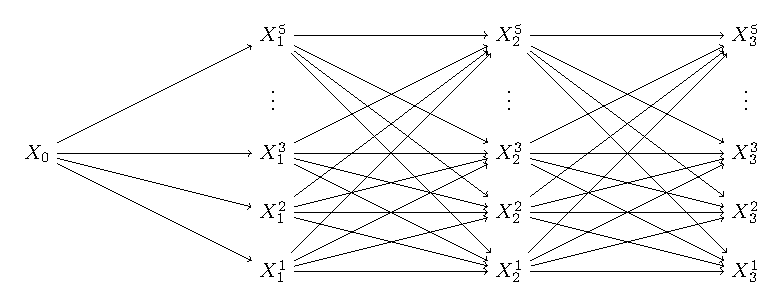
\includegraphics{stohastic_mesh_vector.eps}
    \caption{Стохастическая сетка для $b = 5$ и $m = 3$}
    \label{fig:stochastic_mesh}
\end{figure}

Этот метод работает гораздо быстрее, чем метод случайных деревьев: сложность и по времени, и по памяти составляет $O(mb)$. Недостатком являются трудоёмкие вычисления в многомерном случае: в отличие от случайного дерева, для обсчёта которого нужно лишь уметь вычислить $h_t(X_t)$ (для традиционного примера максимум-опциона на покупку $h_t(X_t) = \left(\max(X_t) - K\right)^+$, если $X_t$ -- вектор стоимостей базовых активов в момент $t$), для стохастических сеток нужно точно вычислять $\rho_n(i, j)$.

% section mesh_estimator (end)

\section{Метод наименьших квадратов} % (fold)
\label{sec:classic_approaches:least_squares}

Несколько отличающийся от двух предыдущих вариант --- метод оценки с помощью линейной регрессии \cite{Longstaff2001}. Согласно формулировке \eqref{eq:option-recursive}, в каждый момент $t$ мы хотим знать математическое ожидание стоимости удержания (неисполнения) опциона при условии его текущего состояния. Классический инструмент для оценки условного математического ожидания --- это линейная регрессия. Будем оценивать стоимость удержания опциона следующим образом:

\begin{equation}\label{eq:lsm_continuation}
\E\left(V_i(X_i)\middle\vert X_{i-1} = x\right) \approx \sum_{r=1}^M \beta_{ir} \psi_r(x) = \beta_i^\mathsf{T}\psi(x).
\end{equation}
Здесь $\psi(x) = \left(\psi_1(x), \dots, \psi_M(x)\right)^\mathsf{T}$ --- это набор регрессоров, используемых для построения оценки. В оригинальной статье использовались полиномы Лагера (\cite[секция~2.2 на стр.~122]{Longstaff2001}) и для построения регрессии использовались только те траектории, на которых опцион в $i-1$-й момент времени находился в деньгах.

Используемая здесь сетка похожа на ту, что была в методе стохастической сетки: моделируем несколько траекторий, тем самым получая нужный набор примеров (см. рис.~\ref{fig:least_squares}). Коэффициенты $\beta$ оцениваются по методу наименьших квадратов. 

\begin{figure}[t]
    \centering
    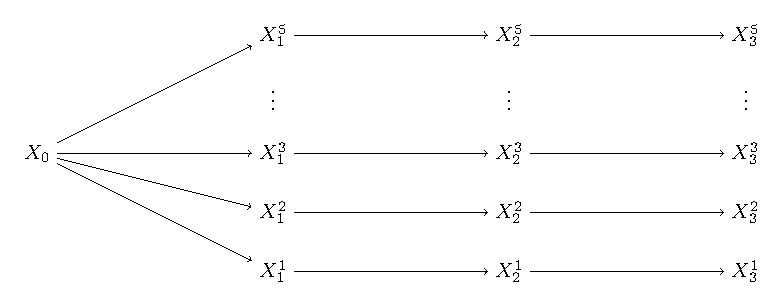
\includegraphics{stohastic_mesh_vector_phase_0.eps}
    \caption{Стохастическая сетка для метода наименьших квадратов, $b = 5$ и $m = 3$}
    \label{fig:least_squares}
\end{figure}

Для каждого узла сетки теперь возможно оценить стоимость удержания опциона по выражению \eqref{eq:lsm_continuation} и понять, было бы оптимальным решением исполнить опцион в этот момент (если выручка от немедленного исполнения превосходит стоимость удержания опциона, то оптимальным решением будет исполнить опцион, иначе -- оставить его для исполнения в какой-либо из последующих моментов). После того, как установлены моменты оптимального исполнения опциона для каждой из исходных траекторий, составлявших сетку, стоимость опциона на траектории устанавливается равной выплате, полученной в оптимальный для этой траектории момент исполнения. Итоговая стоимость опциона оценивается усреднением по всем траекториям. Более формально эта процедура изложена в алгоритме~\ref{alg:least_squares_estimation}.

\begin{algorithm}[h]
    \SetAlgorithmName{Алгоритм}{алгоритм}{Список алгоритмов}
    \SetKwInput{KwData}{Входные данные}
    \SetKwInput{KwResult}{Результат}
    \SetKw{KwTo}{до}\SetKwFor{For}{Для}{\string:}{}%
    \KwData{сетка из $b$ промоделированных траекторий состояния базового актива $X_n^i,\;\;n\in 1\mathbin{:}m,\;i \in 1\mathbin{:}b$}
    \KwResult{$\Vhat$ -- оценка стоимости опциона}
    
    положим стоимость опциона равной выплате по нему в последний момент исполнения:\\$C_i \leftarrow h_{t_m}\left(X_m^i\right)$, $C = \left(C_1, \dots, C_b\right)^{\mathsf T}$\;
    \For{$n\leftarrow m-1$ \KwTo $1$}{
        % дисконтируем стоимость опциона: $C \leftarrow e^{-r\deltat} \cdot C$\tcc*[r]{если $h_t$ уже дисконтированная, этого делать не нужно}\;
        $X_i \leftarrow S_n^i$, $X = \left(X_1, \dots, X_b\right)^{\mathsf T}$\;
        выплаты по исполнении опциона $P_i \leftarrow h_{t_n}\left(X_n^i\right)$, $P = \left(P_1, \dots, P_b\right)^{\mathsf T}$\;
        строим линейную регрессию $C$ на $X$ через набор базисных функций $\psi$ по всем тем примерам, где опцион в деньгах:\\ $\beta \leftarrow \argmin_{\beta'\in\R^M} \norm{\left({\beta'}^\mathsf{T}\psi(X_i) - C_i\right)_{\left\{i \middle\vert P_i > 0\right\}}}^2$\;
        стоимость удержания опциона $H_i = \beta^\mathsf{T}\psi(X_i)$\;
        \For{всех $i$ таких, что $P_i > H_i$}{
            $C_i \leftarrow P_i$\;
        }
    }
    $\Vhat \leftarrow \frac{1}{b}\sum_{i=1}^b C_i$

    \caption{Оценка стоимости опциона по методу наименьших квадратов}
\label{alg:least_squares_estimation}
\end{algorithm}

В \cite{Glasserman2004} указано, что метод наименьших квадратов можно считать частным случаем метода стохастической сетки со специальным выбором весов. Тем не менее, часто эти подходы рассматриваются по отдельности.

% \subsubsection{Численные результаты} % (fold)
% \label{ssub:lsm_numerical_results}

% Метод наименьших квадратов был реализован для $\psi_1(x) = x, \psi_2(x) = x^2$. Результаты представлены на рис.~\ref{fig:classical_methods} и в табл.~\ref{tbl:lsm_estimators}.

% \begin{table}
%     % \renewcommand{\arraystretch}{0.75}
%     \centering
%     \caption{Оценки методом наименьших квадратов}
%     \begin{tabular}{rrrrr}
%         $b$&$\Vhat$&$\mathrm{sd}\Vhat$&$\mathrm{se}\Vhat$&$\mathrm{bias}\Vhat$\\\hline
%         10&26.870&6.324&6.521&2.527\\
%         20&25.957&4.774&4.822&0.459\\
%         50&25.312&2.877&2.877&0.001\\
%         100&24.965&2.106&2.129&0.099\\
%         200&24.795&1.480&1.557&0.235\\
%         500&24.772&0.918&1.050&0.258\\
%         1000&24.731&0.636&0.840&0.301\\
%     \end{tabular}
%     \label{tbl:lsm_estimators}

%     \footnotesize
%     Результаты приведены для ширины сетки $b = 10, 20, 50, 100, 200, 500, 1000$.\\\vspace{-0.3\baselineskip}Расшифровку обозначений см. в выражении~\eqref{eq:table_labels}.
% \end{table}

% chapter classic_approaches_to_option_pricing (end)